\chapter{Arhitektura i dizajn sustava}
		
		%\textbf{\textit{dio 1. revizije}}\\

		%\textit{ Potrebno je opisati stil arhitekture te identificirati: podsustave, preslikavanje na radnu platformu, spremišta podataka, mrežne protokole, globalni upravljački tok i sklopovsko-programske zahtjeve. Po točkama razraditi i popratiti odgovarajućim skicama:}
	%\begin{itemize}
	%	\item 	\textit{izbor arhitekture temeljem principa oblikovanja pokazanih na predavanjima (objasniti zašto ste baš odabrali takvu arhitekturu)}
		%\item 	\textit{organizaciju sustava s najviše razine apstrakcije (npr. klijent-poslužitelj, baza podataka, datotečni sustav, grafičko sučelje)}
	%	\item 	\textit{organizaciju aplikacije (npr. slojevi frontend i backend, MVC arhitektura) }		
%	\end{itemize}

		Arhitektura našeg sustava dijeli se na tri podsustava: baza podataka, web aplikacija i web poslužitelj.
			
		\underbar{Web preglednik} program je koji služi kao posrednik između korisnika i web poslužitelja. Korisniku omogućuje pregled web-stranica te multimedijskih sadržaja vezanih uz njih. Svaka stranica pisana je u nekom kodu koji prosječnom korisniku ništa ne znači, no kako je svaki internetski preglednik ujedno i prevoditelj, on prikazuje stranicu u obliku koja je svakome razumljiva. Na taj način korisnik šalje zahtjeve web poslužitelju.
		
		\underbar{Web poslužitelj} kao osnovnu zadaću ima ostvarivanje komunikacije između klijenta i aplikacije.  Ta komunikacija ostvarena je HTTP-om (engl. HyperText Transfer Protocol). Upravo je web poslužitelj temelj rada web aplikacije. On ju pokreće i prosljeđuje zahtjeve zaprimljene od web preglednika.
		
		\underbar{Web aplikacija} koju korisnik koristi obrađuje njegove zahtjeve. Ukoliko je potrebno za obradu zahtjeva, web aplikacija komunicira s poslužiteljem baze podataka koji joj dohvaća i prosljeđuje potrebne podatke. Potom web aplikacija vraća odgovor u obliku HTML dokumenta te web preglednik to prikazuje korisniku u odgovarajućem formatu.
		
		Za izradu naše web aplikacije odlučili smo se za programski jezik Python s njegovim radnim okvirom Django. Koristili smo Bootstrap, HTML, CSS i JavaScript za prikaz web-stranica. Baza podataka implementirana je kroz PostgreSQL. Arhitektura sustava temeljit će se na MVT (eng. \textit{Model View Template}) obrascu koji se tek marginalno razlikuje od MVC (eng. \textit{Model View Controller}) obrasca. S obzirom da je MVT koncept podržan od strane Djanga, na raspolaganju su nam gotovi predlošci te nam znatno olakšavaju razvoj web aplikacije.
	
		Zahvaljujući nezavisnosti razvoja pojedinih djelova aplikacije možemo jednostavnije ispitivati i razvijati sustav, kao i dodavati nova svojstva. Kao što se može pretpostaviti, MVT koncept sastoji se od triju komponenti. "Model" i "View" na strani su poslužitelja i nisu vidljivi korisniku, dok je "Template" vidljiv na korisničkoj strani. "Model" je središnja jkomponenta sustava te pristupa bazi podataka. Pravilno formatira podatke dobivene od strane "View"-a te ih prosljeđuje bazi podataka i obrnuto. "View" prima podatke i zahtjeve kao što su "POST" i "GET" s klijentske strane. Također pravilno formatira primljene podatke te komunicira s druge dvije komponente MVT koncepta. "Template" služi za prikazivanje sadržaja na web-stranici. Sadrži statičke i dinamičke definicije prikaza sadržaja.
		
		\begin{figure} [!h] %ovaj [!h] je potreban za fiksiranje slike točno na ovo mjesto u pdf-u.
			\centering
			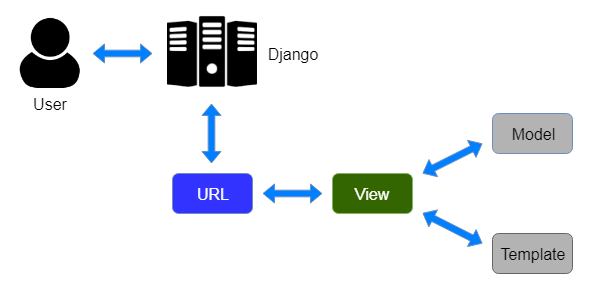
\includegraphics[width=0.7\linewidth]{slike/MVT}
			\caption{MVT koncept}
			\label{fig:mvt}
		\end{figure}
		
		\eject		

				
		\section{Baza podataka}
			
		Koristimo relacijsku bazu podataka napisanu u jeziku SQL te je ostvarujemo kroz postgreSQL. Pregled cijele baze imamo preko programa pgAdmin 4. Tamo gledamo spremaju li se promjene, jesu li one smislene te dodajemo specifičan sadržaj za testiranje. Django preko komponente "Model" pristupa bazi te je ona strukturno cijela sadržana u datoteci models.py.
		
			\subsection{Opis tablica}
			
				
				\begin{longtabu} to \textwidth {|X[10, l]|X[6, l]|X[20, l]|}
					
					\hline \multicolumn{3}{|c|}{\textbf{Korisnik}}	 \\[3pt] \hline
					\endfirsthead
					
					\hline \multicolumn{3}{|c|}{\textbf{Korisnik}}	 \\[3pt] \hline
					\endhead
					
					\hline 
					\endlastfoot
					
					\cellcolor{LightGreen}korisnikid & INT	&  	Redni broj korisnika (primarni ključ). 	\\ \hline
					email	& VARCHAR &  Korisnikov e-mail  (maksimalno 100 znakova). \\ \hline
					korisnickoime & VARCHAR & Ime koje predstavlja korisnika na stranici (maksimalno 20 znakova). \\ \hline 
					lozinka & VARCHAR & Korisnikova lozinka za prijavu (maksimalno 20 znakova).  \\ \hline 
					razinaautoriteta & INT & Razina autoriteta korisnika. 1 predstavlja korisnika, a 2 admina. \\ \hline 
					adresa & VARCHAR & Korisnikova adresa (maksimalno 100 znakova). \\ \hline 
					rodendan & DATE & Datum korisnikovog rođendana.  \\ \hline 
					datumregistracije & DATE & Datum korisnikove registracije.  \\ \hline 
					adresaprivatna & BOOL & Želi li korisnik javno prikazati svoju adresu na svome profilu? \\ \hline 
					rodendanprivatan & BOOL & Želi li korisnik javno prikazati svoj rođendan na svome profilu?   \\ \hline
					datumregistracije
					privatan & BOOL & Želi li korisnik javno prikazati svoj datum registracije na svome profilu?  \\ \hline 
					ime & VARCHAR &  Korisnikovo ime (maksimalno 50 znakova).  \\ \hline 
					prezime  & VARCHAR & Korisnikovo prezime (maksimalno 50 znakova).  \\ \hline 
					dozvoljenpristup & BOOL & Ima li korisnik dozvoljen pristup stranici?  \\ \hline 
					brojracuna & VARCHAR & Broj bankovnog računa korisnika. (21 znak)  \\ \hline
					\cellcolor{LightBlue} 
					profilnaid & INT & Redni broj medijske datoteke koja sadrži korisnikovu profilnu fotografiju. (strani ključ)  \\ \hline 
					emailprivatan & BOOL & Želi li korisnik javno prikazati svoj e-mail na svome profilu?   \\ \hline 
					imeprezimeprivatno & BOOL & Želi li korisnik javno prikazati svoje ime i prezime na svome profilu?  \\ \hline 					
					
				\end{longtabu}
			
				\begin{longtabu} to \textwidth {|X[10, l]|X[6, l]|X[20, l]|}
				
				\hline \multicolumn{3}{|c|}{\textbf{Komentar}}	 \\[3pt] \hline
				\endfirsthead
				
				\hline \multicolumn{3}{|c|}{\textbf{Komentar}}	 \\[3pt] \hline
				\endhead
				
				\hline 
				\endlastfoot
				
				\cellcolor{LightGreen}komentarid & INT	&  	Redni broj komentara (primarni ključ). 	\\ \hline
				sadrzaj	& VARCHAR &  Tekstualni sadržaj komentara (maksimalno 300 znakova). \\ \hline
				\cellcolor{LightGreen}
				korisnikid & INT & Redni broj korisnika koji je ostavio komentar. (strani ključ) \\ \hline 
				\cellcolor{LightBlue}
				pricaid & INT & Redni broj priče na kojoj je ostavljen komentar. (strani ključ) \\ \hline 	
				
				\end{longtabu}
			
				\begin{longtabu} to \textwidth {|X[10, l]|X[6, l]|X[20, l]|}
					
				\hline \multicolumn{3}{|c|}{\textbf{KorisnikDislajkaopricu}}	 \\[3pt] \hline
				\endfirsthead
				
				\hline \multicolumn{3}{|c|}{\textbf{KorisnikDislajkaopricu}}	 \\[3pt] \hline
				\endhead
				
				\hline 
				\endlastfoot
				
				\cellcolor{LightBlue}
				korisnikid & INT & Redni broj korisnika koji je označio sa "ne sviđa mi se". (strani ključ) \\ \hline 
				\cellcolor{LightBlue}
				pricaid & INT & Redni broj priče koja je označena sa "ne sviđa mi se". (strani ključ) \\ \hline 	
					
				\end{longtabu}
			
				\begin{longtabu} to \textwidth {|X[10, l]|X[6, l]|X[20, l]|}
					
					\hline \multicolumn{3}{|c|}{\textbf{KorisnikLajkaopricu}}	 \\[3pt] \hline
					\endfirsthead
					
					\hline \multicolumn{3}{|c|}{\textbf{KorisnikLajkaopricu}}	 \\[3pt] \hline
					\endhead
					
					\hline 
					\endlastfoot
					
					\cellcolor{LightBlue}
					korisnikid & INT & Redni broj korisnika koji je označio priču sa "sviđa mi se". (strani ključ) \\ \hline 
					\cellcolor{LightBlue}
					pricaid & INT & Redni broj priče koja je označena sa "sviđa mi se". (strani ključ) \\ \hline 	
					
				\end{longtabu}
			
			\begin{longtabu} to \textwidth {|X[10, l]|X[6, l]|X[20, l]|}
				
				\hline \multicolumn{3}{|c|}{\textbf{Maketa}}	 \\[3pt] \hline
				\endfirsthead
				
				\hline \multicolumn{3}{|c|}{\textbf{Maketa}}	 \\[3pt] \hline
				\endhead
				
				\hline 
				\endlastfoot
				
				\cellcolor{LightGreen}maketaid & INT	&  	Redni broj makete (primarni ključ). 	\\ \hline
				\cellcolor{LightBlue}
				dimenzije & VARCHAR & Dimenzije makete u centimetrima. \\ \hline 
				\cellcolor{LightBlue}
				mediaid & INT & Redni broj medijske datoteke koja sadrži sliku makete. (strani ključ) \\ \hline 	
				
			\end{longtabu}
		
			\begin{longtabu} to \textwidth {|X[10, l]|X[6, l]|X[20, l]|}
				
				\hline \multicolumn{3}{|c|}{\textbf{MaketaKupljena}}	 \\[3pt] \hline
				\endfirsthead
				
				\hline \multicolumn{3}{|c|}{\textbf{MaketaKupljena}}	 \\[3pt] \hline
				\endhead
				
				\hline 
				\endlastfoot
				
				\cellcolor{LightGreen}id & INT	&  	Redni broj kupovine makete (primarni ključ). 	\\      \hline			
				kolicina & INT & Broj istih maketa kupljenih pri ovoj narudžbi. \\ \hline 
				\cellcolor{LightBlue}
				maketaid & INT & Redni broj navedene makete. (strani ključ) \\ \hline 
				\cellcolor{LightBlue}
				materijalid & INT & Redni broj materijala od kojeg je izgrađena navedena maketa. (strani ključ) \\ \hline 	
				\cellcolor{LightBlue}
				maketaid & INT & Redni broj transakcije u pitanju. (strani ključ) \\ \hline 
				
			\end{longtabu}
		
			\begin{longtabu} to \textwidth {|X[10, l]|X[6, l]|X[20, l]|}
				
				\hline \multicolumn{3}{|c|}{\textbf{Materijal}}	 \\[3pt] \hline
				\endfirsthead
				
				\hline \multicolumn{3}{|c|}{\textbf{Materijal}}	 \\[3pt] \hline
				\endhead
				
				\hline 
				\endlastfoot
				
				\cellcolor{LightGreen}materijalid & INT	&  	Redni broj materijala (primarni ključ). 	\\      \hline			
				ime & VARCHAR & Ime materijala (maksimalno 100 znakova). \\ \hline 
				
			\end{longtabu}
		
			\begin{longtabu} to \textwidth {|X[10, l]|X[6, l]|X[20, l]|}
			
			\hline \multicolumn{3}{|c|}{\textbf{Media}}	 \\[3pt] \hline
			\endfirsthead
			
			\hline \multicolumn{3}{|c|}{\textbf{Media}}	 \\[3pt] \hline
			\endhead
			
			\hline 
			\endlastfoot
			
			\cellcolor{LightGreen}mediaid & INT	&  	Redni broj medijske datoteke (primarni ključ). 	\\      \hline			
			putdodatoteke & VARCHAR & Relativni put do datoteke u repozitoriju. \\ \hline 
			
			\end{longtabu}
				
				\begin{longtabu} to \textwidth {|X[10, l]|X[6, l]|X[20, l]|}
				
				\hline \multicolumn{3}{|c|}{\textbf{MultimedijaPriče}}	 \\[3pt] \hline
				\endfirsthead
				
				\hline \multicolumn{3}{|c|}{\textbf{MultimedijaPriče}}	 \\[3pt] \hline
				\endhead
				
				\hline 
				\endlastfoot
						
				poredakuprici & INT & Broj u poretku po kojem se slaže multimedija u nekoj priči. \\ \hline 
				\cellcolor{LightBlue}
				mediaid & INT & Redni broj medijske datoteke u pitanju. (strani ključ) \\ \hline 
				\cellcolor{LightBlue}
				pricaid & INT & Redni broj priče u pitanju. (strani ključ) \\ \hline 
				
			\end{longtabu}
		
		\begin{longtabu} to \textwidth {|X[10, l]|X[6, l]|X[20, l]|}
			
			\hline \multicolumn{3}{|c|}{\textbf{NapravljenaOd}}	 \\[3pt] \hline
			\endfirsthead
			
			\hline \multicolumn{3}{|c|}{\textbf{NapravljenaOd}}	 \\[3pt] \hline
			\endhead
			
			\hline 
			\endlastfoot
						
			cijena & FLOAT & Cijena makete napravljene od specifičnog materijala. \\ \hline 
			\cellcolor{LightBlue}
			maketaid & INT & Redni broj makete u pitanju. (strani ključ) \\ \hline 
			\cellcolor{LightBlue}
			materijalid & INT & Redni broj materijala u pitanju. (strani ključ) \\ \hline 
			
		\end{longtabu}
	
			\begin{longtabu} to \textwidth {|X[10, l]|X[6, l]|X[20, l]|}
				
				\hline \multicolumn{3}{|c|}{\textbf{Priča}}	 \\[3pt] \hline
				\endfirsthead
				
				\hline \multicolumn{3}{|c|}{\textbf{Priča}}	 \\[3pt] \hline
				\endhead
				
				\hline 
				\endlastfoot
				
				\cellcolor{LightGreen}pricaid & INT	&  	Redni broj priče (primarni ključ). 	\\      \hline			
				naslovprice & VARCHAR & Naslov priče (maksimalno 100 znakova). \\ \hline 
				datumprice & DATE & Datum objave priče. \\ \hline
				objavljena & BOOL & Je li priča objavljena? \\ \hline 
				maketaprodana & BOOL & Je li maketa iz priče (ako priča sadrži maketu) prodana? \\ \hline 
				\cellcolor{LightBlue}
				maketaid & INT & Redni broj makete u pitanju. (strani ključ) \\ \hline 
				\cellcolor{LightBlue}
				autorid & INT & Redni broj autora priču. (strani ključ) \\ \hline 
				\cellcolor{LightBlue}
				predloziopricuid & INT & Redni broj osobe koja je predložila priču. (strani ključ) \\ \hline 
				\cellcolor{LightBlue}
				tekstpriceid & INT & Redni broj medijske datoteke koja sadrži tekst priče. (strani ključ) \\ \hline 
				
			\end{longtabu}
		
			\begin{longtabu} to \textwidth {|X[10, l]|X[6, l]|X[20, l]|}
			
			\hline \multicolumn{3}{|c|}{\textbf{Tema}}	 \\[3pt] \hline
			\endfirsthead
			
			\hline \multicolumn{3}{|c|}{\textbf{Tema}}	 \\[3pt] \hline
			\endhead
			
			\hline 
			\endlastfoot
			
			\cellcolor{LightGreen}temaid & INT	&  	Redni broj teme (primarni ključ). 	\\      \hline			
			ime & VARCHAR & Ime teme (maksimalno 100 znakova). \\ \hline 		
			\cellcolor{LightBlue}
			teksttemeid & INT & Redni broj medijske datoteke koja sadrži tekst teme. (strani ključ) \\ \hline 
			
		\end{longtabu}
	
		\begin{longtabu} to \textwidth {|X[10, l]|X[6, l]|X[20, l]|}
			
			\hline \multicolumn{3}{|c|}{\textbf{Transakcija}}	 \\[3pt] \hline
			\endfirsthead
			
			\hline \multicolumn{3}{|c|}{\textbf{Transakcija}}	 \\[3pt] \hline
			\endhead
			
			\hline 
			\endlastfoot
			
			\cellcolor{LightGreen}transakcijaid & INT	&  	Redni broj transakcije(primarni ključ). 	\\      \hline			
			ime & VARCHAR & Ime kupca (maksimalno 100 znakova). \\ \hline 
			prezime & VARCHAR & Prezime kupca (maksimalno 100 znakova). \\ \hline 
			adresa & VARCHAR & Adresa kupca (maksimalno 100 znakova). \\ \hline 	
			brojracuna & VARCHAR & Broj računa kupca ( 21 znak). \\ \hline 	
			ukupaniznos & FLOAT & Ukupan iznos transakcije \\ \hline 
			
		\end{longtabu}
	
		\begin{longtabu} to \textwidth {|X[10, l]|X[6, l]|X[20, l]|}
			
			\hline \multicolumn{3}{|c|}{\textbf{CustomMaketa}}	 \\[3pt] \hline
			\endfirsthead
			
			\hline \multicolumn{3}{|c|}{\textbf{CustomMaketa}}	 \\[3pt] \hline
			\endhead
			
			\hline 
			\endlastfoot
			
			\cellcolor{LightGreen}custommaketaid & INT	&  	Redni broj makete na zahtjev (primarni ključ). 	\\      \hline			
			datumotvaranja
			zahtjeva & DATE & Datum slanja zahtjeva za maketu. \\ \hline 
			datumzatvaranja
			zahtjeva & DATE & Datum zaključavanja zahtjeva za maketu. \\ \hline 
			ponudenacijena & FLOAT & Ponuđena cijena za navedenu maketu. \\ \hline 
			prihvaceno & BOOL & Je li korisnik prihvatio ponuđenu cijenu? \\ \hline 
			\cellcolor{LightBlue}
			korisnikid & INT & Redni broj korisnika koji šalje zahtjev. (strani ključ) \\ \hline 
			\cellcolor{LightBlue}
			tekstzahtjevaid & INT & Redni broj medijske datoteke koja sadrži tekst zahtjeva. (strani ključ) \\ \hline 	
			
			
		\end{longtabu}
		
			
			
			
			\subsection{Dijagram baze podataka}
			\vspace{\baselineskip}
			\vspace{\baselineskip}
			\vspace{\baselineskip}
			\vspace{\baselineskip}
			\vspace{\baselineskip}
			\vspace{\baselineskip}
			\vspace{\baselineskip}
			\vspace{\baselineskip}
			\vspace{\baselineskip}
			\vspace{\baselineskip}
				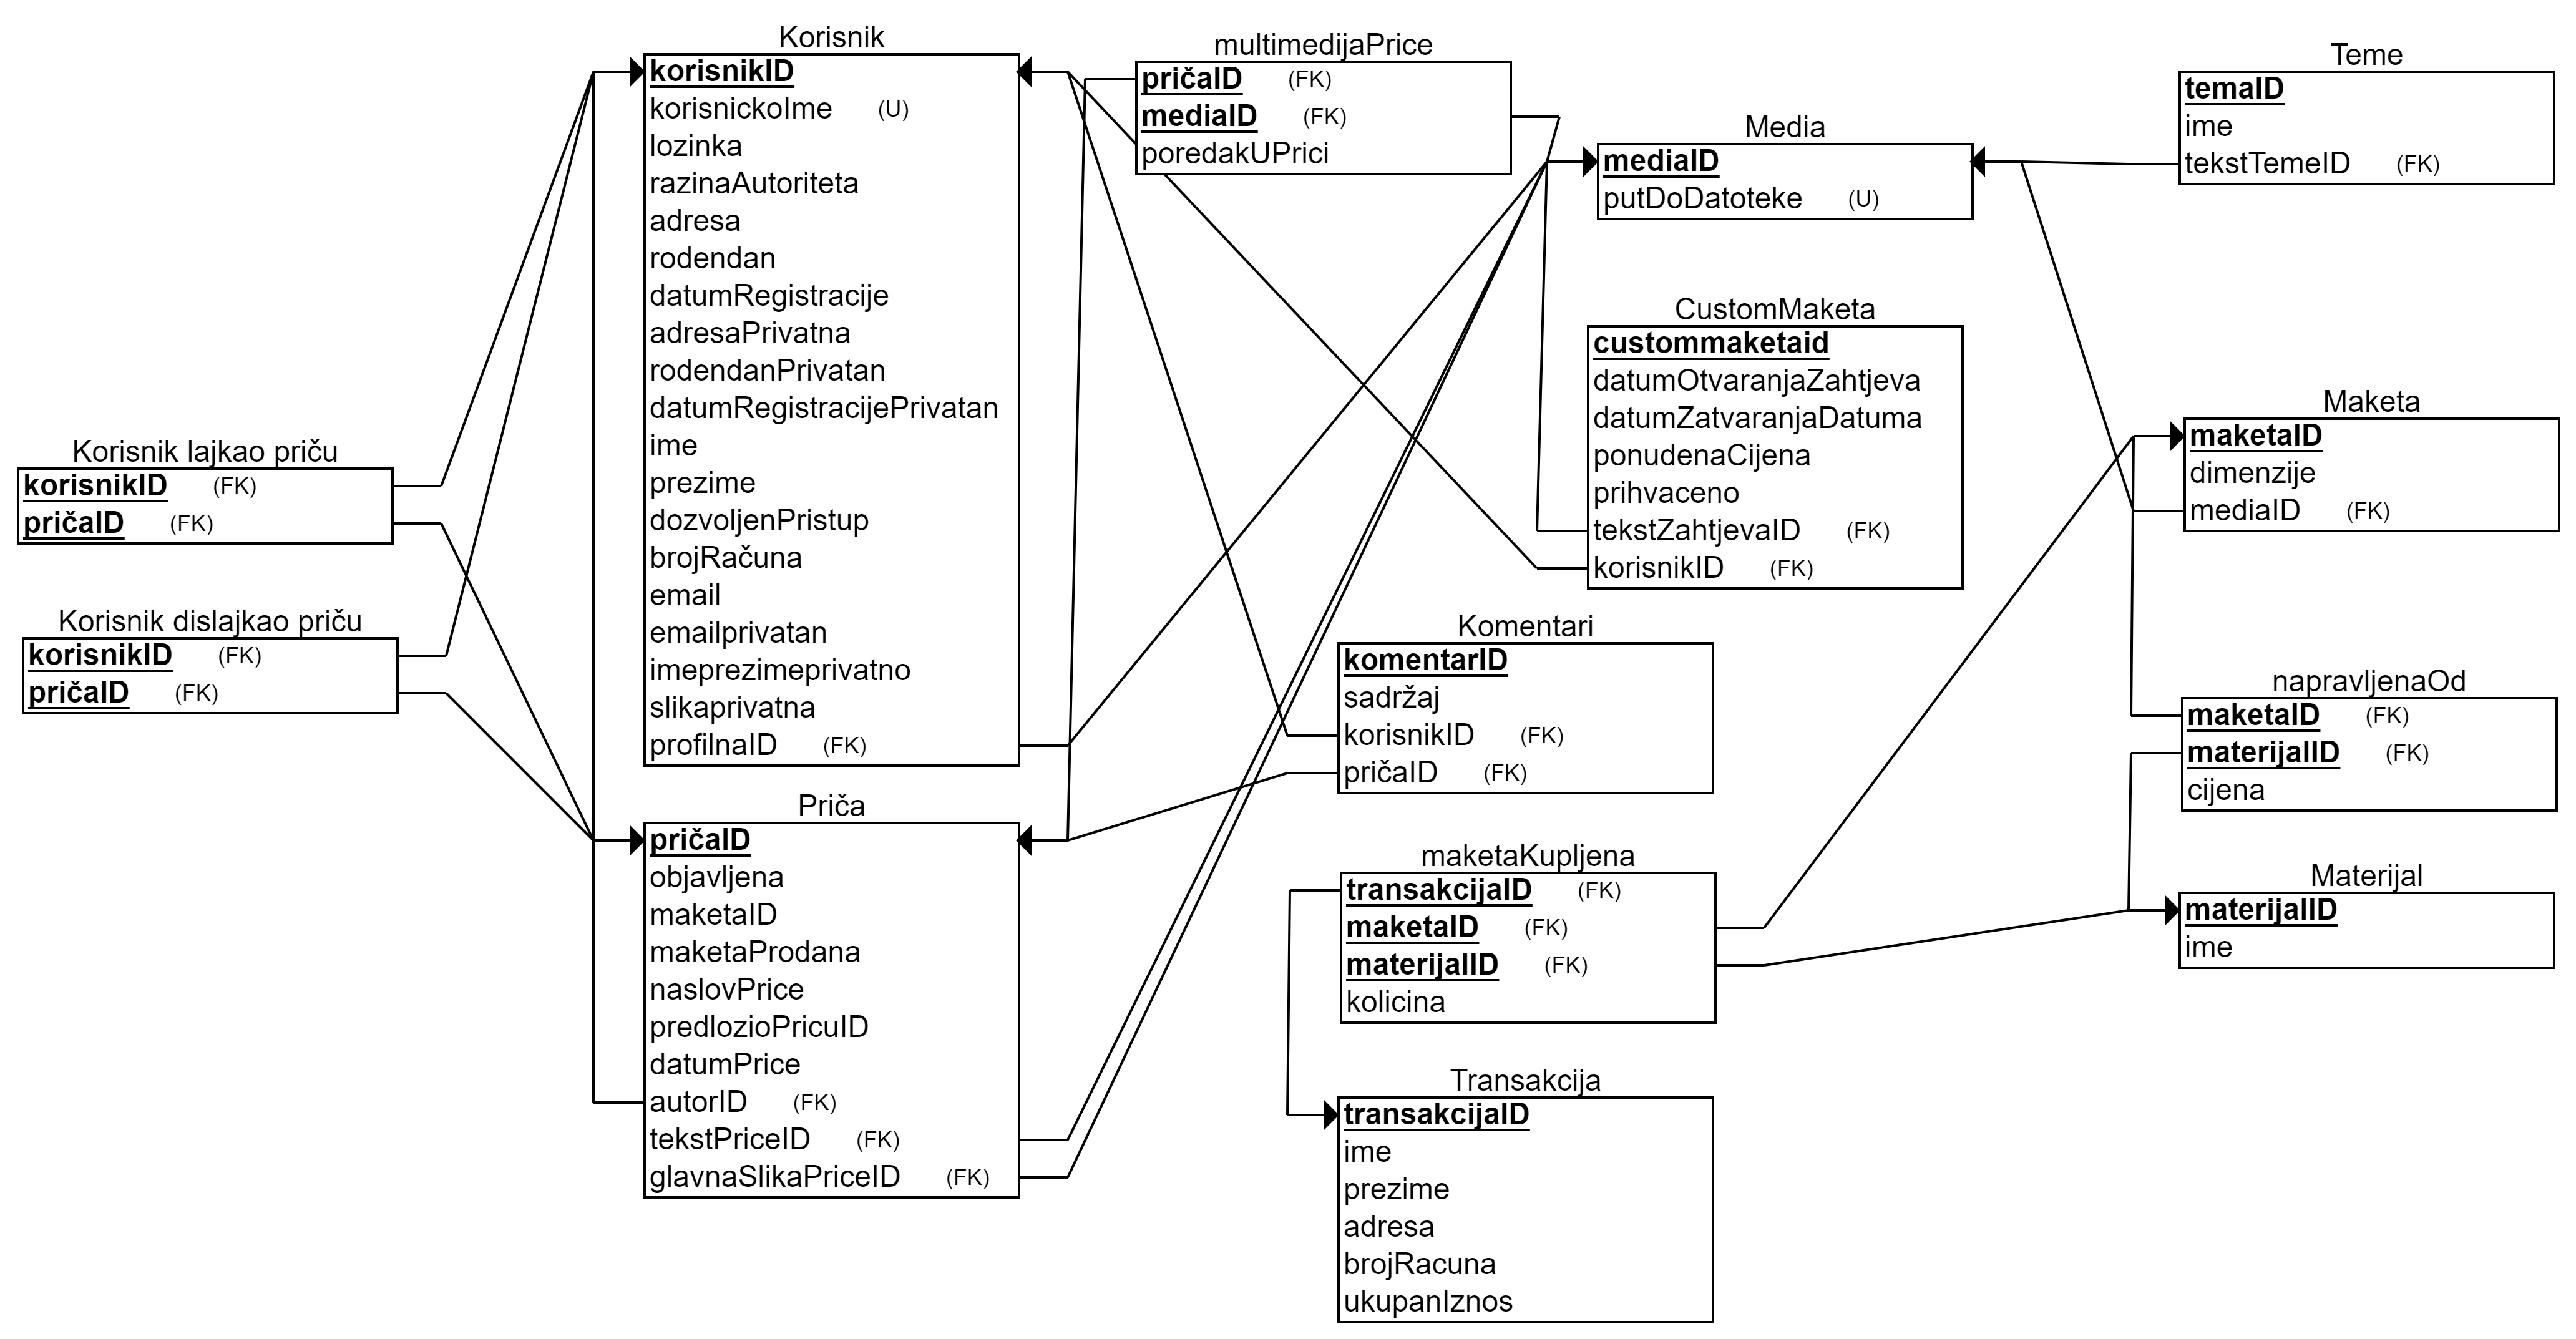
\includegraphics[width=1\linewidth]{slike/bazaRelShem}
			
			\eject
			
			
		\section{Dijagram razreda}
		
		Slike 4.2, 4.3 i 4.4 predstavljaju implementaciju razreda korištenih u backendu za prijenos podataka u korištenoj MTV arhitekturi. Slika 4.2 sadrži sve korištene razrede koji predstavljaju View tipove. Na slici 4.3 prikazane su Data Transfer Object tipovi podataka koji primaju podatake iz modela.  Slika 4.4 prikazuje razred modela onako kako su zapamćeni u bazi podataka te služe za direktnu interakciju s njom. WeTriedContext predstavlja sveukupan sadržaj korištene baze podataka.


		\begin{figure}[!h]
			\centering
			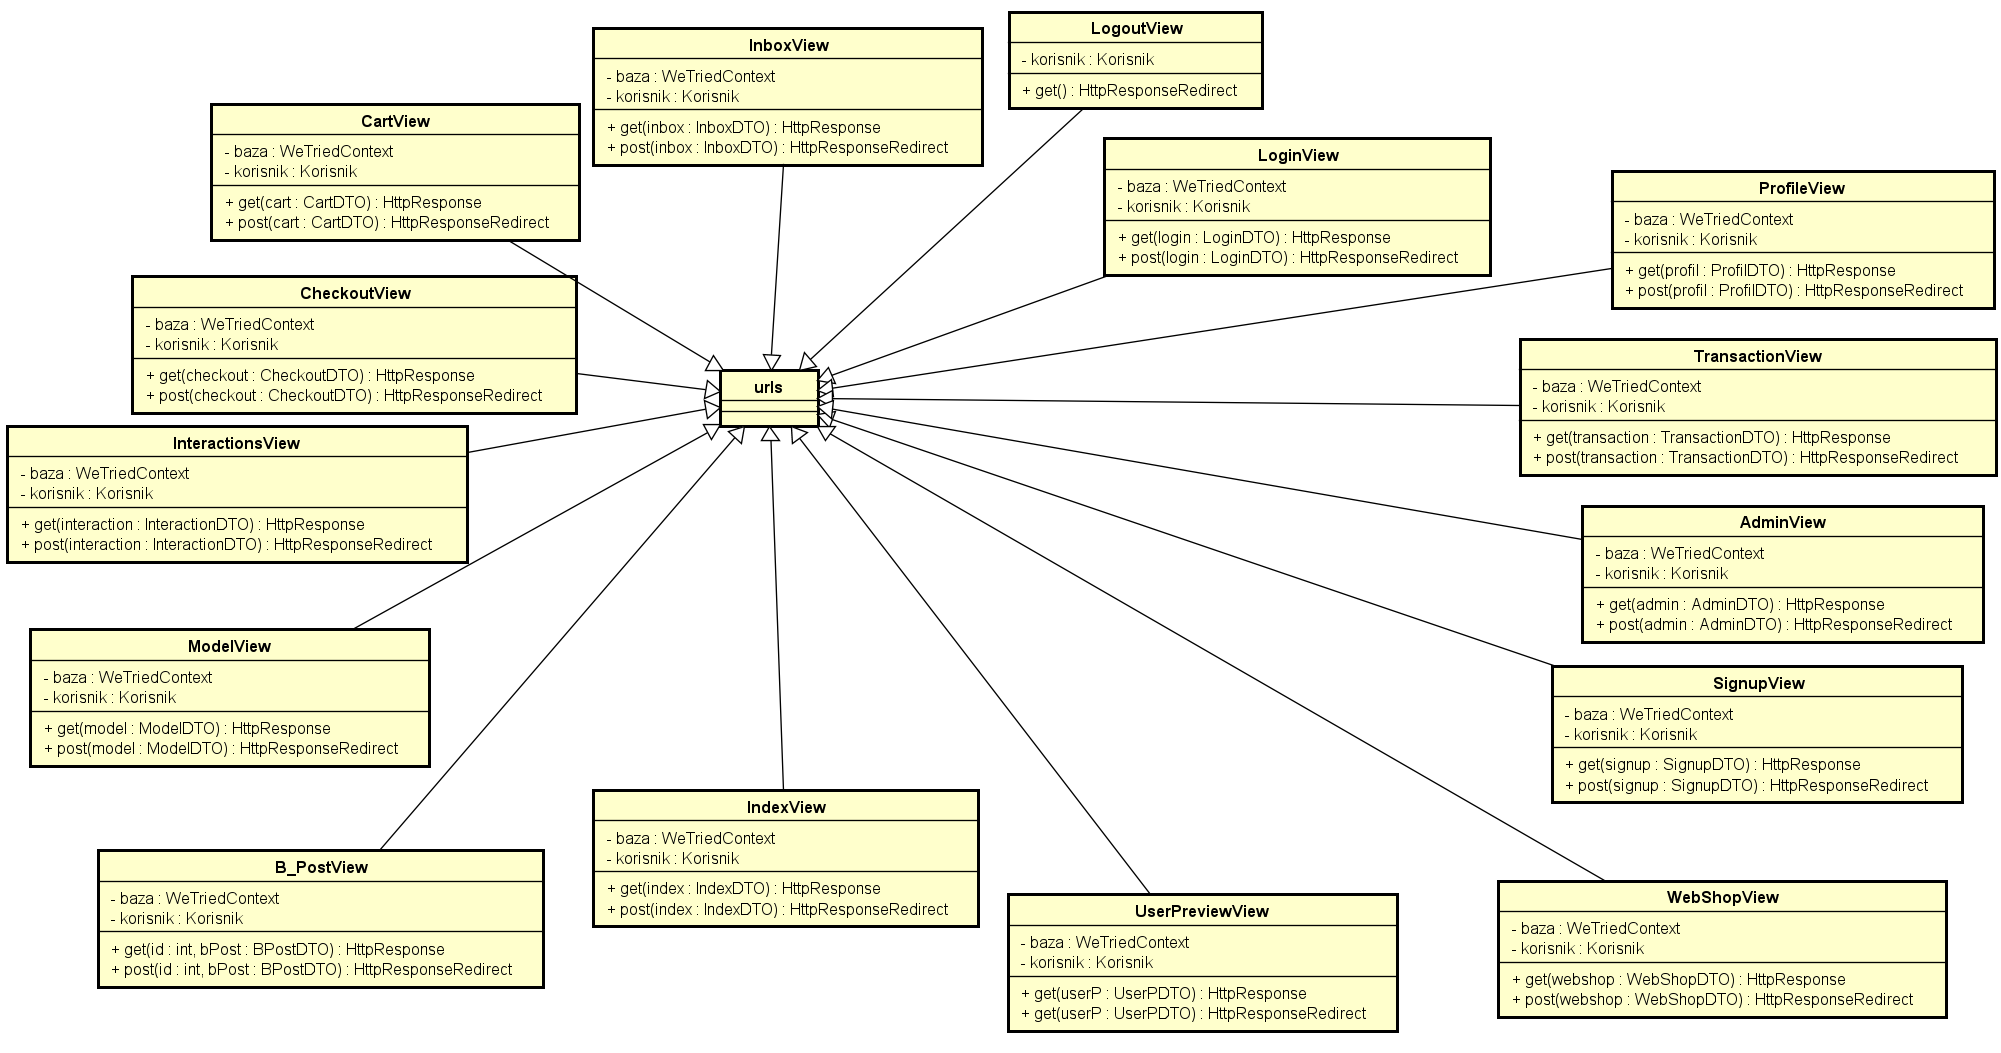
\includegraphics[width=1.1\linewidth, height=0.4\textheight]{slike/dijagram_razreda_1}
			\caption{Dijagram razreda - Views}
			\label{fig:dijagramrazreda1}
		\end{figure}
		
		
		
		
		\begin{figure}
			\centering
			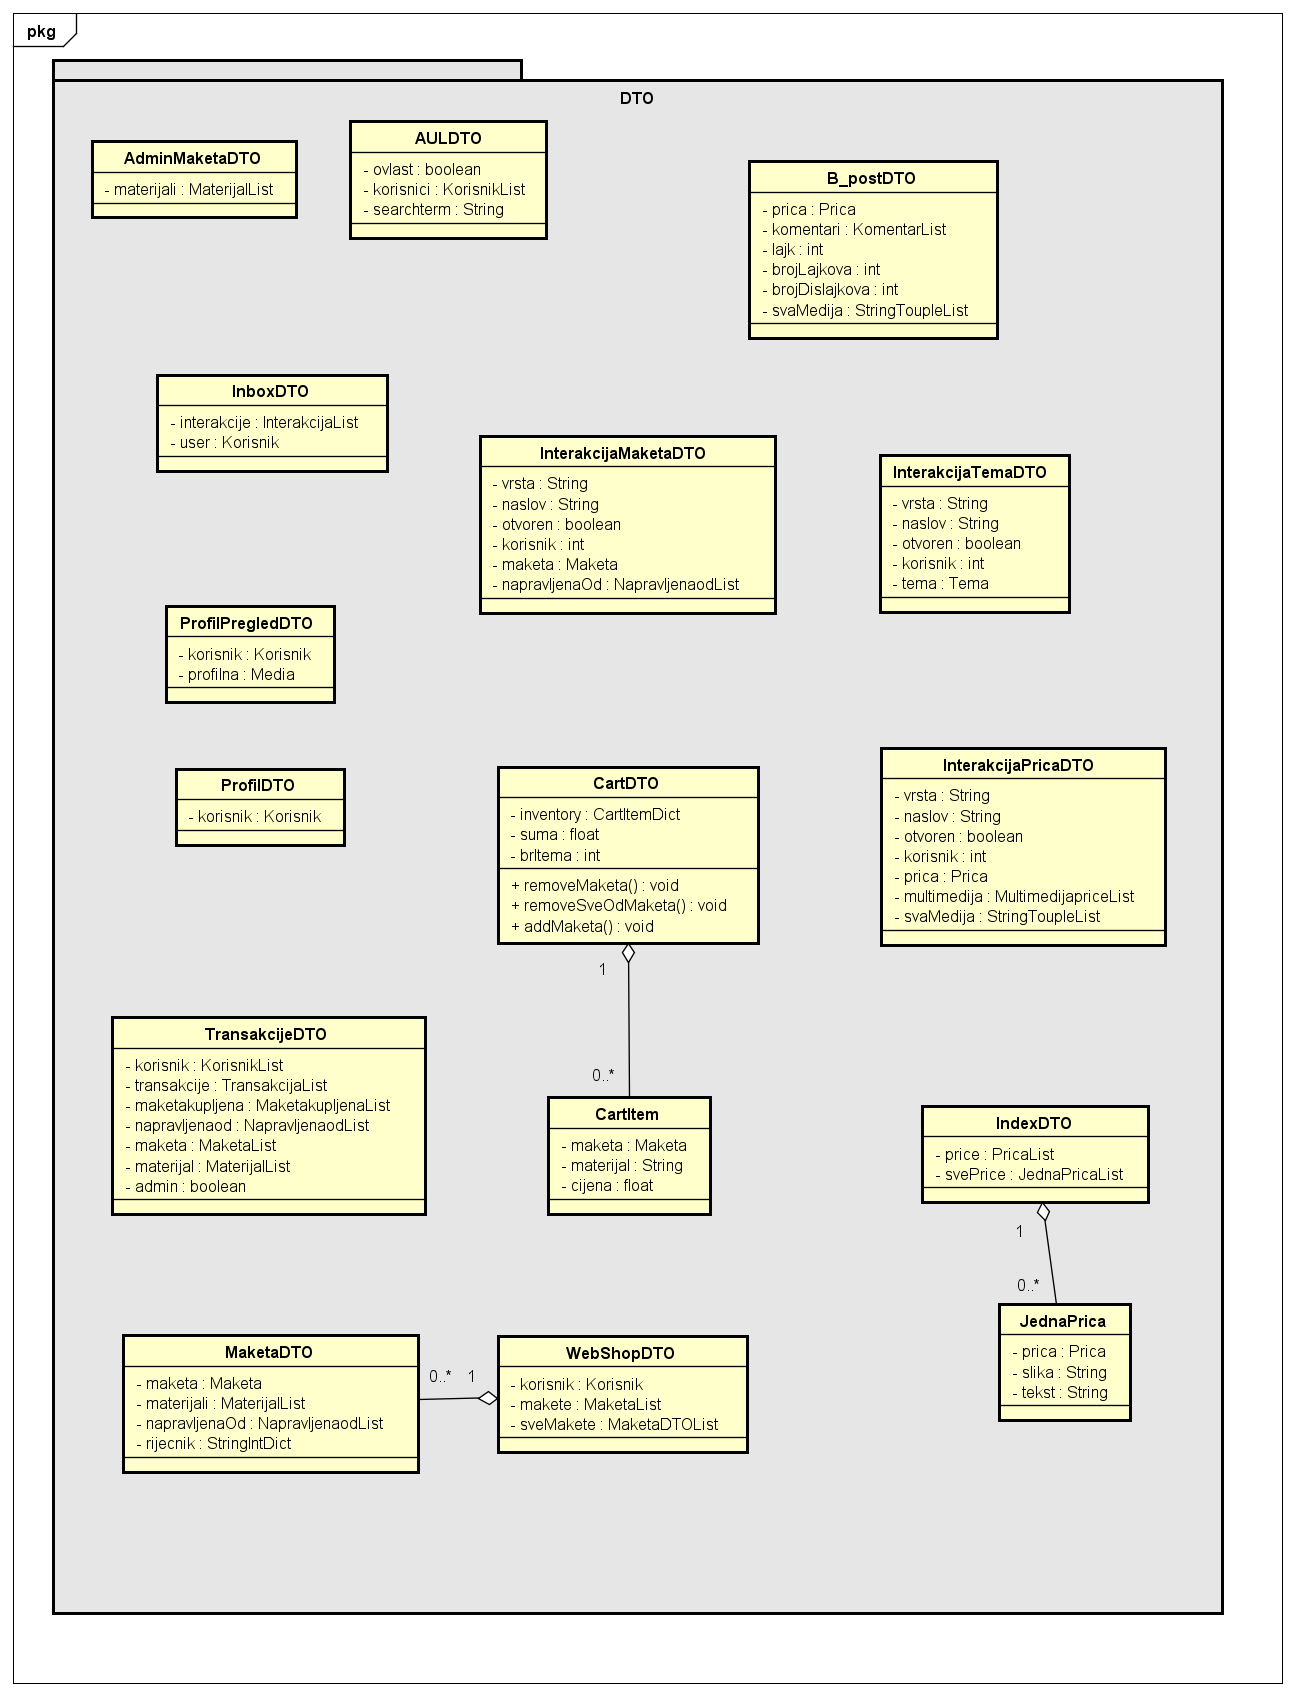
\includegraphics[width=1.0\linewidth]{slike/dijagram_razreda_2}
			\caption{Dijagram razreda - DTO}
			\label{fig:dijagramrazreda2}
		\end{figure}
		\begin{figure}
			\centering
			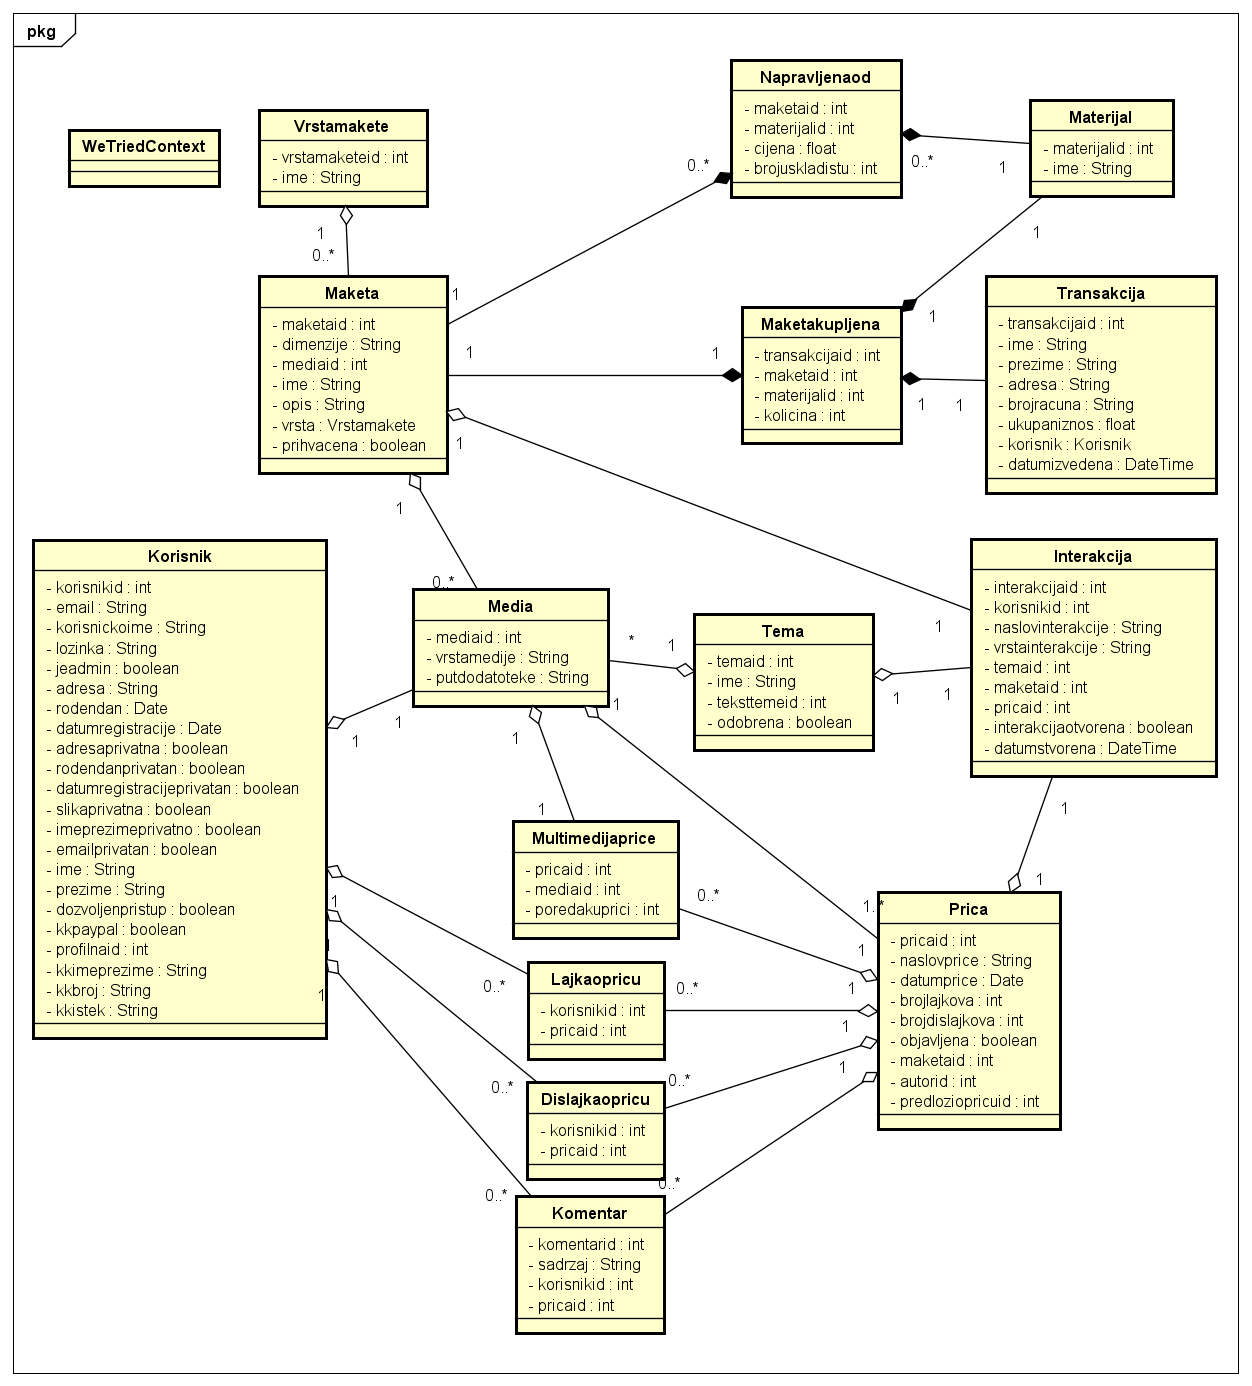
\includegraphics[width=1.0\linewidth]{slike/dijagram_razreda_3}
			\caption{Dijagram razreda - Models}
			\label{fig:dijagramrazreda3}
		\end{figure}
			\eject
